\chapter{Implementation} \label{chap:implementation}

\section{Overview}

This chapter presents the implementation of \namesecureworkstation/, a secure workstation. We use Qubes OS, an existing system described previously, as the base of our implementation. Qubes OS uses virtualization to provide the ability to run isolated applications. The implementation uses separate browser instances for each site-aggregate. Each browser instance runs in a different virtual machine providing isolation among different site-aggregates, which is the idea behind Site Aggregate Isolation policy.

Traffic from each browser instance is routed through an intermediate proxy virtual machine. This proxy VM implements a HTTP/HTTPS filter using a man-in-the-middle proxy server called {\tt mitmproxy}. The proxy server filters requests from each browser instance to enforce the other policies presented previously. To support these policies, Quboid requires additional information from the websites about their site-aggregate names, external resource requirements, etc. that it obtains from HTTP response headers.

\afterpage{\clearpage
\begin{figure}[p]
\centering
    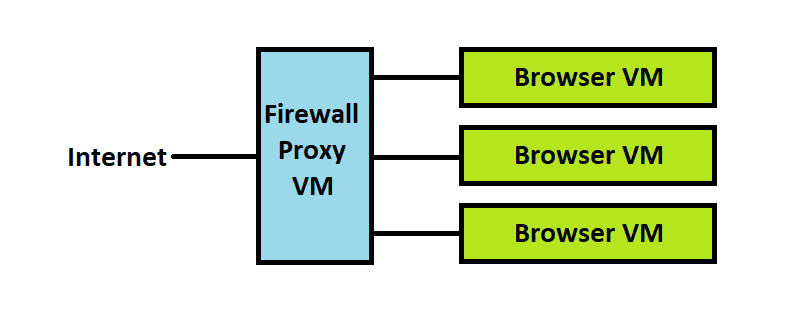
\includegraphics[width=1.0\textwidth]{design_overview.png}
    \caption{Isolation among different site-aggregates in enforced by using a separate browser instance per site-aggregate. Traffic from different browser instances is routed through an intermediate proxy virtual machine. The proxy VM runs a HTTP/HTTPS filter to filter requests from the browsers to provide isolation and enforce policies presented in this paper.}
   \label{fig:wannacry}
\end{figure}
\clearpage}

Finally, the workstation's user interface is implemented in the form of a single-application window manager. Each browser instance is displayed full-screen with no overlapping content with browser instances belonging to other site-aggregates. The interface also consists of a reserved area which is dedicated to displaying the site-aggregate of the active browser instance as well as any other system prompts. This ensures a strict separation between system content and website content.

\section{Isolation using Qubes OS}

We chose to use Qubes OS as the base for our system because of the strong isolation guarantees it provides among the different virtual machines. Browser instances are opened in separate isolated VMs and are limited to showing web pages from the same site-aggregate. Even if attacks are to exploit a browser bug to compromise the virtual machine the browser is running in, the damage is limited to the webpages from the same site-aggregate as the original website. The attack can not steal any information from other virtual machines. 

We use Firefox web browser to open webpages. The browser is configured to minimize communication with websites other than the website the user is visiting. To increase usability, a Quboid secure workstation plugin is installed in the browser. This plugin also assists the system by providing seamless switching and creation of new browser instances in case the user navigates to a webpage of a different site-aggregate. The plugin adds an additional option to open a link into a new VM when the user opens the context menu by right-clicking on the link.

The browser instances are opened in Qubes disposable VMs (DispVM). A new DispVM is created based on a preexisting template. The root filesystem of such a VM is ephemeral. Once the browser instance is closed, all changes are rolled back and the DispVM is destroyed. Thus, each browser instance is opened using a fresh image of the template runs in isolation of all other instances. This is helpful in the scenario that if one of the disposable VMs gets compromised, the damage is limited to that VM. All the state associated with that VM is destroyed as soon it is shut down.

\subsection{Other Approaches}

\paragraph{Xen Project:} Out first attempt at providing isolation was to implement a custom solution on top of Xen, a popular Linux-based hypervisor. However we soon realized the difficulty of running small lightweight virtual machines and the lack of a graphical user interface. Vanilla Xen is well-suited for running generic virtual machines in a server based settings. However, the system we envisioned was intended to be used as a workstation running applications running in lightweight virtual machines. Without a lot of modifications, it would have been impossible to achieve these goals in Xen by itself. Qubes OS on the other hand uses Xen as its base hypervisor and presents a workstation-like environment which proved ideal for our use case.

\paragraph{Custom Hypervisor:} Another approach we could have tried was to write a hypervisor customized for our needs. However, the cost of implementing a new bug-free hypervisor which can satisfy all our needs was prohibitive. Additionally, solutions such as Qubes OS and Xen have been around for a while and are well-maintained. They have been audited several times for bugs in their implementation. For a custom hypervisor to remain bug-free, its implementation would either have to be too simple to satisfy our needs or would require several hours of auditing which would have been difficult. A plausible alternative could be to write a machine-verifiable hypervisor customized for our needs. Such a hypervisor could have machine-checkable proof that it satisfies a relatively simple specification and provide a strong guarantee of being free of bugs. This approach remains unexplored.

\paragraph{Google Chrome Browser:} Google Chrome, a popular web browser, approaches the isolation problem by running its tabs in a sandboxed environment. Access restrictions are applied to a tab's rendering engine. The engine draws into an off-screen bitmap which is then presented to the user by the browser process. Each tab runs in a separate process in its own sandbox. This approach provides much of the guarantees that Qubes provides in terms of isolation. However, the problem it doesn't solve is controlled execution of untrusted files. If the user downloads a malicious file and executes it, the file will not be executed inside the sandbox. Using Qubes OS to execute untrusted files in an isolated VM solves this problem.

\section{Proxy Filter VM}

The browser virtual machines don't enforce any policies by themselves. Instead all internet traffic is routed through an intermediate proxy virtual machine. This VM enforces all the filter rules such as Site Aggregate Isolation, etc. It allows only HTTP and HTTPS traffic through. It analyzes the HTTP headers in the responses and restricts access to URLs and resources that are disallowed by any of the policies.

HTTPS connections are usually end-to-end encrypted. That means, by default the proxy VM shouldn't be able to view the contents of the request and response. To overcome this limitation, the proxy VM acts as the man-in-the-middle server between the actual target and the user. The proxy VM decrypts and re-encrypts the traffic in order to analyze and enforce the filter policies. It uses a software called mitmproxy, a web proxy written in Python.

mitmproxy generates a custom CA certificate which is then installed in the browsers as a trusted CA. Any websites that the browsers access through mitmproxy appear to be signed with a self-signed certificate by the custom CA. The mitmproxy is responsible for verifying and enforcing SSL/TLS security and inspecting the actual server certificates for validity and expiration, since this can no longer be enforced by the browsers themselves.

In order to enforce Site Aggregate policy, the proxy must obtain additional information from the website. This information includes the site-aggregate name of the website, the list of external resources needed, the allowed site-aggregates with whom the website is allowed to communicate, etc. This information is contained in the form of new HTTP response headers.

The site-aggregate name is received from the {\tt Site-Aggregate} header field. The site-aggregate name must be web-requestable URLs. The proxy must verify the name by sending a request to the site-aggregate name and checking that the requested page is in the same site-aggregate.
List of allowed URLs should be checked against the {\tt Site-Aggregate-Pattern} header field. List of allowed resources and exit destinations should be checked against the {\tt Cross-Site-Aggregate-Resource-Pattern} and {\tt Exit-Pattern} header fields.

\subsection{Other Approaches}

As opposed to redirecting the traffic through a proxy, it is also possible to enforce the policy rules in the browser itself. We decided against that approach for the following reason - in the event that a browser VM is compromised, it will leave the network exposed. The compromised VM would then be able to display and request any external resources from the internet including those belonging to different site-aggregates. There are several attacks known to exploit bugs in browser systems such as Adobe Flash or the Javascript engine. Therefore, we decided to move the enforcement away from the browser and into a separate proxy VM.

\section{Site Aggregate Isolation}

The proxy VM has the ability to inspect all traffic going between the users and web servers. The enforcement of the Site Aggregate Isolation policy is achieved by using HTTP headers. The responses from the web server contain information about its site-aggregate name, allowed exit destinations, list of external resources, etc. The proxy VM maintains a list of all the information contained the headers for each virtual machine and uses it to make decisions on whether to allow a request to go through or not.

The following subsections list the introduced HTTP headers and the policies that are used to allow or deny requests using those headers.

\subsection{HTTP Request Headers}

We do not introduce any new HTTP request headers. However, we do require the usage of the existing HTTP Referer Header \cite{rfc-referrer} \cite{mozdev-referrer}.

\paragraph{\texttt{Referer}} The {\tt Referer} header contains the URL of the previous webpage from which a link was followed. This can be used to by webpages to log the URLs from which link back to a webpage. We require the usage of this field on all requests for the purposes of filtering. Web servers must check this header field on all requests and deny any requests for which the {\tt Referer} field is not recognized. This should be enforced specifically for all the internal links of a website. If a webpage is only meant to be accessible by following internal links, access to that webpage should be prohibited from outside sources.

An example of an attack that this might prevent is when a website has a internal API which has been made public by accident. Other websites may be able to take advantage of this by listing that internet API address as an external resource and hence be able to extract information from the API.

\subsection{Resource Integrity Checks}

Several websites use CDN's to deliver scripts or stylesheets. One method to ensure that these external resources have not been tampered with to verify their integrity when they are loaded. In order to support this, a new \texttt{integrity} attribute is included for external scripts and stylesheets. The value of this attribute contains the hashed checksum of the resource to be loaded. The browser can then verify the integrity of this external resource. This method is known as Subresource Integrity \cite{subresource-integrity} \cite{subresource-integrity-2} check, and is already part of a W3C recommendation.

We encourage the use of this attribute on all static external resources to prevent malicious content to be loaded into the webpage.

\subsection{Other Approaches}

The higher level idea behind using HTTP response headers is that of providing additional information about the webpage to the secure workstation. It is possible that this information may be provided in other ways, for example, the website may have an API that provides this information. There was no compelling reason behind usage of HTTP headers as opposed to these other approaches.

It should be ensured when extracting this information that the source of the information is tamper-proof. Malicious external content must not be able to modify this information about the website. Unless the actual webserver is compromised, the source of the information must be kept isolated from the webpage content itself.

\section{Single Application Window Manager}

The final subsystem in the implementation is the user interface. The UI is a single application window manager i.e. it is designed to show exclusively display a single application at a time. This design is inspired by the user interface of smartphones, that only displays one application on the screen at a time. That advantage of this property is that the user is always aware which application is currently being displayed in the foreground. On the other side, it reduces the usability of the system since the user can no longer work on more than one application at the same time. We consider this a reasonable trade-off to create a secure and unambiguous UI.

At all times, there is a reserved area on the screen. This area is used exclusively for system UI elements. The reserved area displays the site-aggregate name of the active browser instance and any prompts by the system. Separation of the display area into a system-only area and an application-only area reduces the risk posed by phishing attacks that appear as system UI.

\begin{figure}[p]
\centering
    \fbox{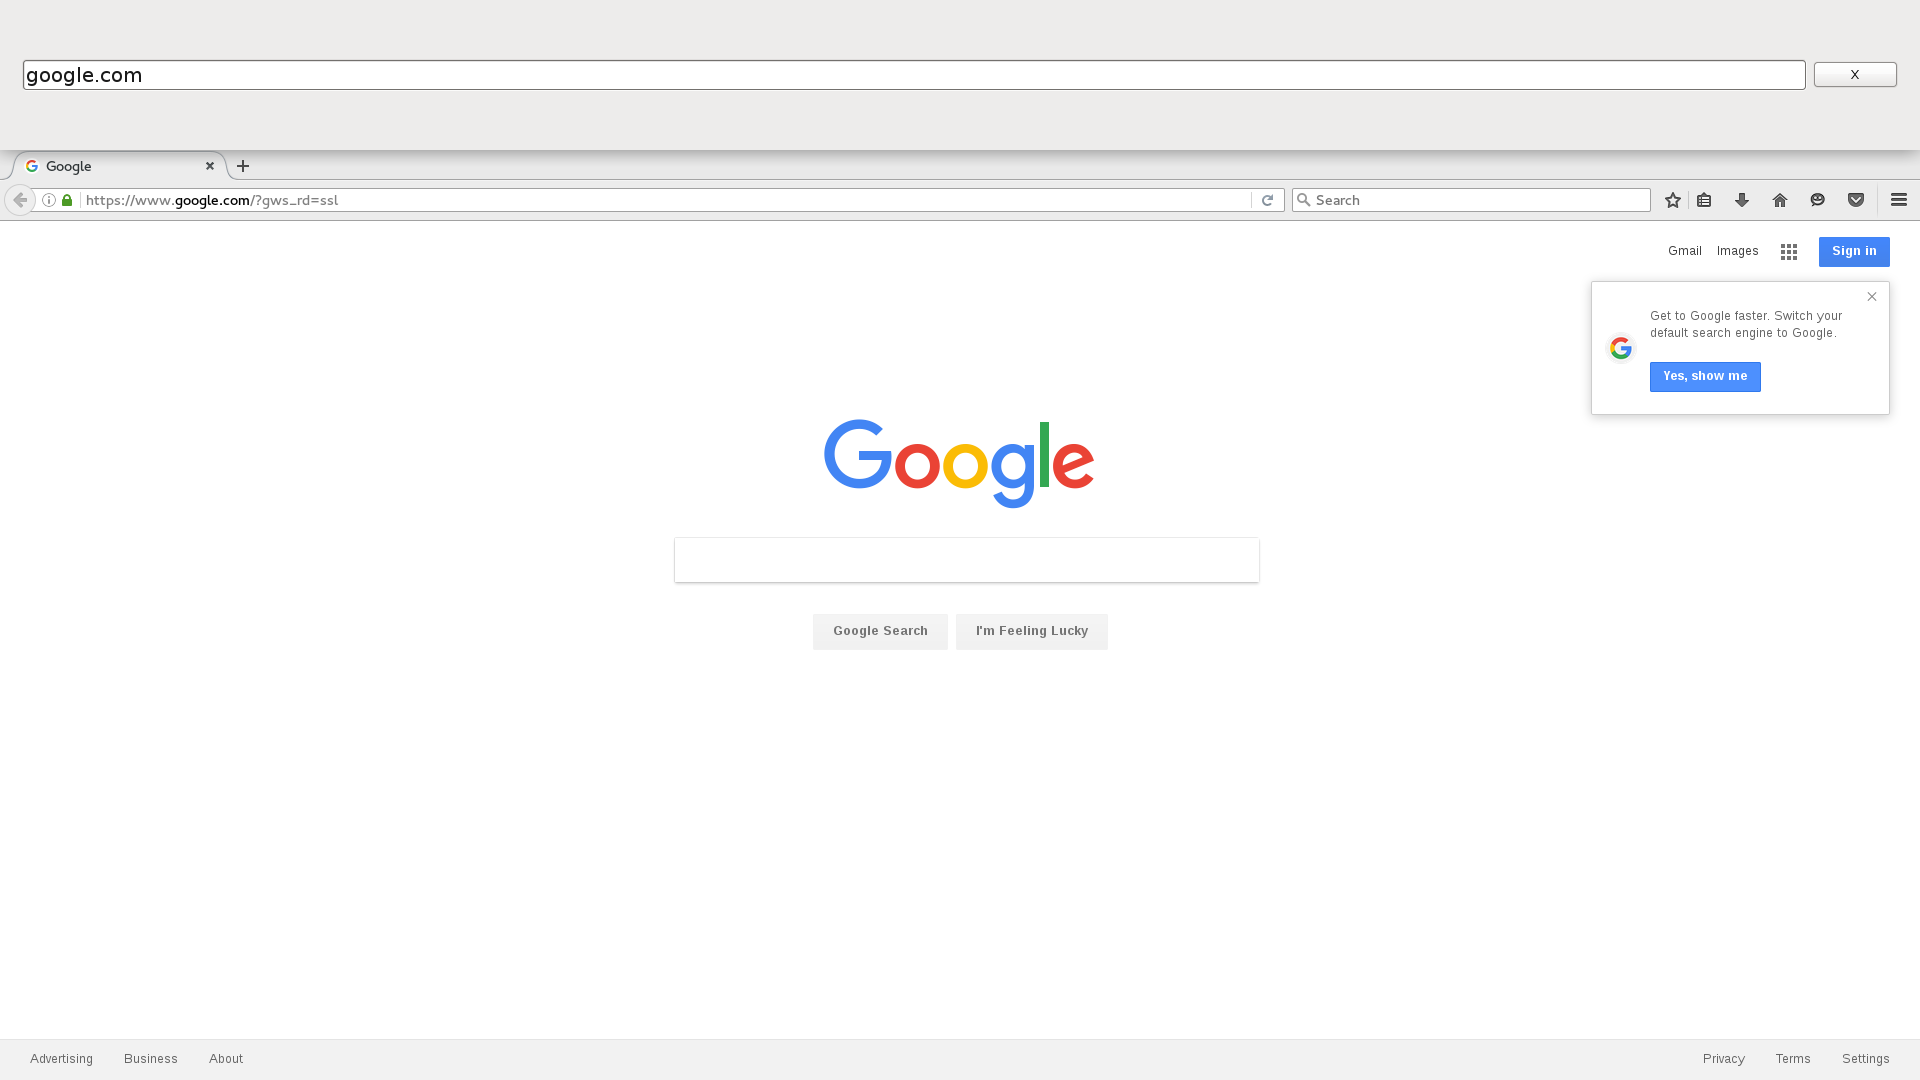
\includegraphics[width=1.0\textwidth]{ui-example.png}}
    \caption{A screenshot of the user interface of the secure workstation implementation. The top bar is a reserved area for the site-aggregate name of the active browser instance and any system prompts. The rest of the screen is used exclusively by a single browser instance.}
   \label{fig:ui-example}
\end{figure}

Figure \ref{fig:ui-example} shows a screenshot of the UI. The top reserved area permanently displays the site-aggregate name of the page visited. The user the ability to open new browser instances by typing in the site-aggregate name of the new website into the top bar.

% \section{Performance}

% We ran dd if=/dev/urandom of=test.html count=100K bs=1 and then downloaded the file
% Download 100k
% On VM:
% 876ms
% 858ms
% 862ms
% 860ms
% 858ms
% 853ms

% Direct:
% 13ms
% 18ms
% 15ms
% 12ms
% 15ms
% 17ms

% With Test server in the proxy also:
% 40ms
% 24ms
% 26ms
% 26ms
% 33ms
% 21ms


% New dispvm opening times
% 2VMs alreadybrunning
% 3.309
% 3.234
% 3.679
% 2.753
% 3.313
% 3.111

% 3VMS
% 5.044
% 5.264
% 3.276
% 3.337
% 23.244
% 3.180
% 3.790
% 3.723

% 4
% 39.874
% 4.652
% 3.113
% 4.210
% 3.711
% 3.620
% 3.402
% 3.605
% 3.312

% 5
% 4.549
% 3.942
% 4.751
% 4.747
% 5.008
% 3.371
% 3.526
% 3.241
% 3.450
% 4.364

% 6
% 4.643
% 4.589
% 4.705
% 5.307
% 4.507

% 4.540

% 4.607

% 4.843

% ~> 10